\documentclass[10pt,aspectratio=169]{beamer}

\usetheme{Madrid}
\usecolortheme{dove}
\setbeamertemplate{navigation symbols}{}
\setbeamertemplate{footline}[frame number]

% Uncomment one of these for presenter mode:
% \usepackage{pgfpages}
% \setbeameroption{show notes on second screen=right}  % dual-screen
% \setbeameroption{show notes}                          % notes as separate pages

\usepackage{booktabs}
\usepackage{amsmath}
\usepackage{xcolor}
\usepackage{tikz}
\usetikzlibrary{arrows.meta, positioning}
\usepackage{graphicx}
\usepackage{colortbl}
\usepackage{array}
\usepackage[round,authoryear]{natbib}

\definecolor{accentblue}{RGB}{0,80,160}
\definecolor{accentred}{RGB}{180,30,30}
\definecolor{lightblue}{RGB}{220,235,255}
\definecolor{wingreen}{RGB}{210,245,210}

\title[Functional Load Forecasting]{Functional Forecasting of Turkish Electricity Load Curves}
\author{Zeynep Bozoklu}
\institute{Thesis Proposal}
\date{\today}

\begin{document}

% ============================================================
% SLIDE 1: TITLE
% ============================================================
\begin{frame}
  \titlepage
  \note{Introduce the thesis topic: applying Functional Data Analysis to forecast Turkey's daily electricity load curve. The core result is that our model beats the official TEİAŞ benchmark by 19\% with near-zero p-value. Walk through 14 slides in roughly 20 minutes.}
\end{frame}

% ============================================================
% SLIDE 2: THE FORECASTING OBJECT
% ============================================================
\begin{frame}{The Forecasting Object: A Daily Load Curve}
  \begin{columns}
    \begin{column}{0.62\textwidth}
      \includegraphics[width=\linewidth]{../output/figs/fda_mean_actual_forecast_all.png}
    \end{column}
    \begin{column}{0.35\textwidth}
      \Large $Y_d(h),\quad h=0,\ldots,23$
      \vspace{0.7em}

      \normalsize
      \begin{itemize}
        \item A single \textbf{curve}, not 24 scalars
        \item Dual-peak shape is stable across all days
        \item Solid = actual;\enspace dashed = official forecast
        \item \textbf{Goal:} forecast tomorrow's full 24-hour profile
      \end{itemize}
    \end{column}
  \end{columns}
  \note{Point to the overnight trough (around hour 4--5) and the broad daytime plateau (hours 9--20). The shape is structurally the same every day; what changes is the level and sharpness. Note how the official forecast (dashed) tracks the actual reasonably well on average but lies systematically below it --- we will quantify this underprediction on the next slide.}
\end{frame}

% ============================================================
% SLIDE 3: WHY ACCURACY MATTERS
% ============================================================
\begin{frame}{Why Accuracy Matters}
  \begin{columns}
    \begin{column}{0.44\textwidth}
      \textbf{Key users (post-2013 liberalisation):}
      \vspace{0.4em}
      \begin{itemize}
        \item \textbf{TEİAŞ} (system operator)\\
              {\small unit commitment, grid scheduling}
        \item \textbf{Generators}\\
              {\small day-ahead market bids on EPIAS}
        \item \textbf{Large consumers}\\
              {\small real-time imbalance penalties}
      \end{itemize}
    \end{column}
    \begin{column}{0.53\textwidth}
      \begin{center}
        \textbf{Systematic underprediction --- official TEİAŞ forecast}\\[0.5em]
        \small
        \begin{tabular}{lrr}
          \toprule
          Year & Official bias & Our bias \\
               & (MWh/hour)    & (MWh/hour) \\
          \midrule
          2023 & $+344$ & $+176$ \\
          2024 & $+585$ & $+34$  \\
          2025 & $+472$ & $+98$  \\
          \midrule
          \textbf{Average} & $\mathbf{+467}$ & $\mathbf{+103}$ \\
          \bottomrule
        \end{tabular}\\[0.4em]
        \small Positive bias = forecast $<$ actual (underprediction).
      \end{center}
    \end{column}
  \end{columns}
  \note{The official forecast always undershoots actual demand. The gap widened sharply in 2024. Our rolling-origin model reduces the average bias by 78\%. Just state the empirical fact --- do not speculate about why the official underpredicts. This table motivates the research question: is there systematic improvement to be had?}
\end{frame}

% ============================================================
% SLIDE 4: RESEARCH QUESTIONS
% ============================================================
\begin{frame}{Research Questions}
  \begin{enumerate}
    \item \textbf{Representation:} Can B-spline smoothing and FPCA represent
          Turkey's daily electricity load curves with negligible information loss?\\
          {\small How many functional principal components suffice?}

    \vspace{0.5em}
    \item \textbf{Forecasting accuracy:} Does a functional VAR model augmented
          with holiday and derivative features statistically outperform the
          official TEİAŞ day-ahead forecast?\\
          {\small Tested by Diebold-Mariano over 1,096 hold-out days, 2023--2025.}

    \vspace{0.5em}
    \item \textbf{Error structure:} Can a data-driven residual correction further
          reduce errors at the morning ramp hours where the base model underperforms?\\
          {\small Does serially correlated error contain exploitable signal?}
  \end{enumerate}
  \note{Three questions, three result sections. Q1 is answered in the FPCA slide (97.3\% variance retained with K=2; K=4 robustness check confirms this). Q2 is the main DM result (+19.2\%, $p \approx 10^{-163}$). Q3 is the residual correction (+46.2\%, wins at all 24 hours including ramp). Keep this slide brief --- it frames what the rest of the talk answers.}
\end{frame}

% ============================================================
% SLIDE 5: LITERATURE  [placeholder -- to be expanded]
% ============================================================
\begin{frame}{Literature Positioning \textcolor{gray}{\small [to be expanded]}}
  \begin{columns}
    \begin{column}{0.48\textwidth}
      \textbf{Functional Data Analysis}
      \vspace{0.2em}
      \begin{itemize}
        \item Ramsay \& Silverman (2005): FDA foundations
        \item Kokoszka \& Reimherr (2017): modern inference
        \item Hyndman \& Ullah (2007): functional forecasting (demographics)
      \end{itemize}
      \vspace{0.4em}
      \textbf{FDA applied to load curves}
      \begin{itemize}
        \item \textit{[to be identified in literature review]}
      \end{itemize}
    \end{column}
    \begin{column}{0.48\textwidth}
      \textbf{Short-term electricity forecasting}
      \vspace{0.2em}
      \begin{itemize}
        \item Classical: ARIMA, exponential smoothing
        \item ML: gradient boosting, neural networks
        \item Xie \& Hong (2016): residual simulation / correction
      \end{itemize}
      \vspace{0.4em}
      \textbf{Gap this thesis fills}
      \begin{itemize}
        \item No FDA study on Turkey's post-liberalisation electricity market
        \item Holiday + derivative features tailored to Turkish market structure
        \item Formal DM testing against operational benchmark
      \end{itemize}
    \end{column}
  \end{columns}
  \note{Placeholder --- the systematic literature review is the primary remaining task. Key message to establish in the final thesis: FDA has been applied to electricity load curves in Western European contexts but not Turkey; and existing Turkish electricity forecasting papers use scalar methods (ARIMA, regression). The contribution is both methodological and empirical (Turkey 2019--2025, post-2013 liberalisation). Add specific paper citations as the review progresses.}
\end{frame}

% ============================================================
% SLIDE 6: THE FDA PIPELINE
% ============================================================
\begin{frame}{From 24 Numbers to a Curve: The FDA Pipeline}
  \vspace{-0.2em}
  \begin{center}
  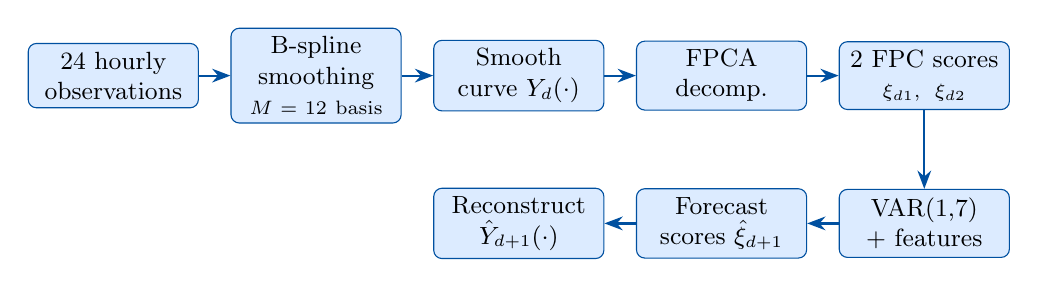
\begin{tikzpicture}[
    node distance=0.45cm and 0.40cm,
    box/.style={rectangle, rounded corners=3pt, draw=accentblue, fill=lightblue,
                text width=1.95cm, align=center, font=\small,
                minimum height=0.78cm, inner sep=3pt},
    arr/.style={-Stealth, thick, accentblue}
  ]
    \node[box] (raw)    {24 hourly\\observations};
    \node[box, right=of raw]    (spline) {B-spline\\smoothing\\{\scriptsize $M=12$ basis}};
    \node[box, right=of spline] (curve)  {Smooth\\curve $Y_d(\cdot)$};
    \node[box, right=of curve]  (fpca)   {FPCA\\decomp.};
    \node[box, right=of fpca]   (scores) {2 FPC scores\\{\scriptsize $\xi_{d1},\;\xi_{d2}$}};

    \node[box, below=1.0cm of scores] (var)   {VAR(1,7)\\$+$ features};
    \node[box, left=of var]           (hatsc) {Forecast\\scores $\hat\xi_{d+1}$};
    \node[box, left=of hatsc]         (recon) {Reconstruct\\$\hat{Y}_{d+1}(\cdot)$};

    \draw[arr] (raw)    -- (spline);
    \draw[arr] (spline) -- (curve);
    \draw[arr] (curve)  -- (fpca);
    \draw[arr] (fpca)   -- (scores);
    \draw[arr] (scores) -- (var);
    \draw[arr] (var)    -- (hatsc);
    \draw[arr] (hatsc)  -- (recon);
  \end{tikzpicture}
  \end{center}
  \vspace{0.5em}
  \begin{columns}
    \begin{column}{0.33\textwidth}
      \centering\small\textbf{B-splines}\\
      preserves shape; enables differentiation
    \end{column}
    \begin{column}{0.33\textwidth}
      \centering\small\textbf{FPCA}\\
      2 scores carry 97.3\% of curve variation
    \end{column}
    \begin{column}{0.33\textwidth}
      \centering\small\textbf{VAR(1,7)}\\
      weekly + daily score dynamics
    \end{column}
  \end{columns}
  \note{Walk through the boxes left to right, then down and back. The core idea: instead of 24 separate forecasting models, we compress to 2 scores, forecast those, and reconstruct the full curve. The B-spline step also lets us compute the derivative of the curve, capturing ramp speed --- a feature we add later. This is the methodological contribution.}
\end{frame}

% ============================================================
% SLIDE 5: DATA
% ============================================================
\begin{frame}{Data}
  \begin{columns}
    \begin{column}{0.55\textwidth}
      \begin{center}
      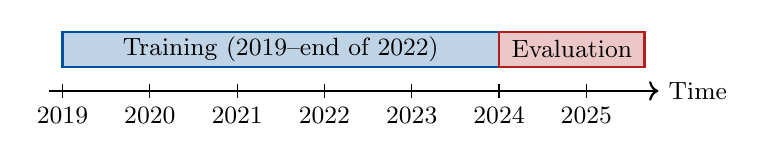
\begin{tikzpicture}[scale=0.88]
        \draw[->, thick] (-0.2,0) -- (8.6,0) node[right,font=\small] {Time};
        \draw[fill=accentblue!25, draw=accentblue, thick]
              (0,0.35) rectangle (6.3,0.85);
        \node[font=\small] at (3.15,0.60) {Training (2019--end of 2022)};
        \draw[fill=accentred!25, draw=accentred, thick]
              (6.3,0.35) rectangle (8.4,0.85);
        \node[font=\small] at (7.35,0.60) {Evaluation};
        \foreach \x/\y in {0/2019, 1.26/2020, 2.52/2021,
                           3.78/2022, 5.04/2023, 6.3/2024, 7.56/2025} {
          \draw (\x,0.1) -- (\x,-0.1) node[below,font=\small] {\y};
        }
      \end{tikzpicture}
      \end{center}
      \vspace{0.4em}
      \small Rolling-origin design: model re-estimated before each\\
      forecast day using only past data. See evaluation slide.
    \end{column}
    \begin{column}{0.42\textwidth}
      \small
      \begin{tabular}{ll}
        \toprule
        \textbf{Series} & \textbf{Source} \\
        \midrule
        Hourly load (MWh) & EPIAS \\
        Official forecast  & TEİAŞ / EPIAS \\
        Holiday calendar   & Official gazette \\
        \bottomrule
      \end{tabular}
      \vspace{0.7em}

      \begin{tabular}{ll}
        \toprule
        \textbf{Item} & \textbf{Value} \\
        \midrule
        Frequency          & Hourly \\
        Coverage           & 2019--2025 \\
        Training curves    & $\approx$1,460 days \\
        Evaluation curves  & 1,096 days \\
        Hourly errors eval & 26,304 \\
        \bottomrule
      \end{tabular}
    \end{column}
  \end{columns}
  \note{Data from EPIAS, Turkey's electricity market operator, via public API. Having both actual load and the official TEİAŞ day-ahead forecast is key: it gives us a directly comparable operational benchmark. The evaluation is deliberately aligned with the operational benchmark: same target days, same hourly load object, and no future information.}
\end{frame}

% ============================================================
% SLIDE 6: FPCA
% ============================================================
\begin{frame}{FPCA: Two Numbers Capture the Curve}
  \begin{columns}
    \begin{column}{0.60\textwidth}
      \includegraphics[width=\linewidth]{../output/figs/eigenfunction_shape_comparison.png}
    \end{column}
    \begin{column}{0.37\textwidth}
      \small
      \begin{tabular}{rrr}
        \toprule
        FPC & Variance & Cumulative \\
        \midrule
        1 & 93.4\% & 93.4\% \\
        2 &  3.9\% & 97.3\% \\
        3 &  1.1\% & 98.4\% \\
        \bottomrule
      \end{tabular}
      \vspace{0.7em}

      \textbf{FPC 1 --- Level}\\
      \small Nearly flat $\Rightarrow$ shifts the whole curve up or down

      \vspace{0.5em}
      \textbf{FPC 2 --- Shape}\\
      \small Positive overnight \& late evening, negative daytime $\Rightarrow$ overnight-vs-daytime contrast

      \vspace{0.6em}
      \textbf{Stability:} three sub-period fits nearly coincide $\Rightarrow$ static FPCA justified

      \vspace{0.4em}
      \textbf{Robustness:} $K=4$ adds $<1$\% further variance; results unchanged
    \end{column}
  \end{columns}
  \note{Top panel (FPC1): nearly flat at 0.13--0.28, meaning a high score uniformly lifts the whole curve --- the ``how much electricity today'' factor. Bottom panel (FPC2): positive at hours 0--5 and 18--23, negative daytime --- the overnight-vs-daytime contrast. Three coloured lines (2019--21, 2020--22, 2022--24) nearly overlap, which empirically justifies using a fixed FPCA basis rather than re-estimating it dynamically.}
\end{frame}

% ============================================================
% SLIDE 7: MODEL
% ============================================================
\begin{frame}{Score Forecasting Model}
  \begin{columns}
    \begin{column}{0.50\textwidth}
      \textbf{Core score dynamics:}
      \[
        \xi_d = a + A_1\xi_{d-1} + A_7\xi_{d-7} + Bz_d + u_d
      \]
      \begin{itemize}
        \item \textbf{Lag 1:} yesterday's level and shape
        \item \textbf{Lag 7:} same-day-last-week seasonality
        \item $z_d$: feature vector (all predetermined)
      \end{itemize}
      \vspace{0.5em}
      \textbf{Reconstruction:}
      \[
        \hat{Y}_{d}(h) = \hat\mu(h)
          + \hat\phi_1(h)\,\hat\xi_{d1}
          + \hat\phi_2(h)\,\hat\xi_{d2}
      \]
      Estimated by OLS, equation-by-equation.
    \end{column}
    \begin{column}{0.47\textwidth}
      \textbf{Feature blocks in $z_d$:}
      \vspace{0.3em}
      \small
      \begin{tabular}{lp{0.54\textwidth}}
        \toprule
        Block & Content \\
        \midrule
        Calendar          & Weekend, annual sine/cosine \\
        \textbf{Holiday}  & Public holidays, Eid, bridge days \\
        Load shape        & Yesterday's mean, peak, range \\
        Rolling avg.      & 7-day, 28-day averages \\
        \textbf{Derivative} & Morning ramp, evening ramp, slope volatility \\
        \bottomrule
      \end{tabular}
      \vspace{0.5em}

      \small Holiday and derivative blocks are the critical additions --- without them the model does not beat the official.
    \end{column}
  \end{columns}
  \note{Lag 7 captures the dominant weekly pattern (Monday resembles last Monday); lag 1 adjusts for recent drift. All features in $z_d$ are known before day $d$ starts --- no lookahead. Derivative features come from differentiating the B-spline curve, capturing how fast demand was changing yesterday. Key message to committee: holiday indicators are non-negotiable; the model is competitive only once they are included.}
\end{frame}

% ============================================================
% SLIDE 8: EVALUATION DESIGN
% ============================================================
\begin{frame}{Evaluation: Rolling-Origin Design}
  \begin{columns}
    \begin{column}{0.55\textwidth}
      \begin{center}
      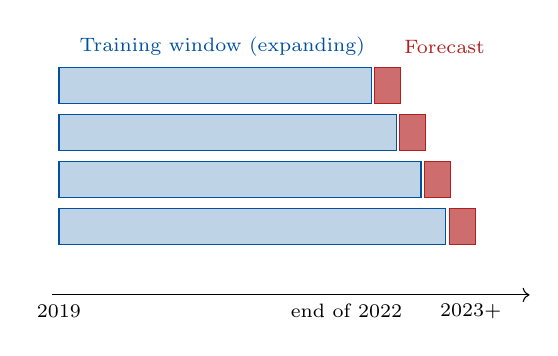
\begin{tikzpicture}[scale=0.83]
        \foreach \i in {1,2,3,4} {
          \pgfmathsetmacro{\tw}{4.4 + \i*0.38}
          \pgfmathsetmacro{\yb}{(5-\i)*0.72}
          \draw[fill=accentblue!25, draw=accentblue]
                (0,\yb) rectangle (\tw, \yb+0.55);
          \draw[fill=accentred!65, draw=accentred]
                (\tw+0.05,\yb) rectangle (\tw+0.45, \yb+0.55);
        }
        \node[font=\scriptsize, accentblue] at (2.5,3.75) {Training window (expanding)};
        \node[font=\scriptsize, accentred]  at (5.9,3.75) {Forecast};
        \node[font=\scriptsize] at (0,  -0.3) {2019};
        \node[font=\scriptsize] at (4.4,-0.3) {end of 2022};
        \node[font=\scriptsize] at (6.3,-0.3) {2023+};
        \draw[->] (-0.1,-0.05) -- (7.2,-0.05);
      \end{tikzpicture}
      \end{center}
      \small Each forecast uses only data dated before that day.\\
      FPCA \emph{and} VAR both re-estimated at every step.
    \end{column}
    \begin{column}{0.42\textwidth}
      \textbf{Metrics:}
      \[
        \text{MAE} = \tfrac{1}{N}\textstyle\sum_{d,h}\lvert e_{dh}\rvert
      \]
      \[
        \text{MAPE} = \tfrac{1}{N}\textstyle\sum_{d,h}\tfrac{\lvert e_{dh}\rvert}{Y_d(h)}
      \]
      \vspace{0.3em}
      \textbf{Significance test:}\\
      Diebold-Mariano (1995)\\
      $H_1$: challenger MAE $<$ official MAE\\
      Pooled (26,304 obs.) + hour-by-hour

      \vspace{0.4em}
      \small A lower MAE number alone is not sufficient evidence.
    \end{column}
  \end{columns}
  \note{Stress the no-leakage principle: the model never sees the future. This mirrors real operational deployment. The Diebold-Mariano test is appropriate because we compare two forecasts for the same target over the same sample --- it accounts for forecast error correlation. Citing Harvey, Leybourne and Newbold (1997) for the small-sample correction is good practice if the committee asks.}
\end{frame}

% ============================================================
% SLIDE 9: MAIN RESULTS
% ============================================================
\begin{frame}{Main Results: DM Confirms the Gains}
  \begin{center}
  \small
  \begin{tabular}{p{0.40\textwidth}rrrrc}
    \toprule
    Model & MAE & MAPE & vs.\ official & DM \\
    \midrule
    Seasonal na\"{i}ve $Y_{d-7}$  & 1912 & 5.13\% & $-57.6\%$ & --- \\
    \textbf{Official (TEİAŞ)}    & \textbf{1214} & \textbf{3.15\%} & ref. & --- \\
    \midrule
    FPCA VAR(1,7)                & 1443 & 3.76\% & $-18.9\%$ & n.s. \\
    $+$ calendar / ramp          & 1238 & 3.26\% & $-2.1\%$  & n.s. \\
    \rowcolor{wingreen}
    $+$ holiday / load-shape     & 1001 & 2.63\% & $+17.5\%$ & *** \\
    \rowcolor{wingreen}
    $+$ derivative features      & \textbf{980} & \textbf{2.56\%}
                                  & $\mathbf{+19.2\%}$ & *** \\
    \midrule
    \rowcolor{wingreen}
    $+$ residual correction      & \textbf{653} & \textbf{1.70\%}
                                  & $\mathbf{+46.2\%}$ & *** \\
    \bottomrule
  \end{tabular}
  \end{center}
  \vspace{0.2em}
  \footnotesize
  DM test vs.\ official: *** $p<0.001$;\enspace n.s. = not significant.
  MAE in MWh/hour; pooled over 26,304 obs.
  \note{Walk the table top to bottom. The seasonal na\"{i}ve shows the floor --- the problem is hard. Pure VAR dynamics are worse than the official. The model turns positive only when holiday and load-shape features are added. Derivative features add another 2 points. Report the DM result explicitly: both the holiday/load-shape row and derivative row beat the official at $p<0.001$, with near-zero p-values ($p \approx 10^{-135}$ and $10^{-163}$ respectively). The main model (bold row) is the baseline contribution; the residual correction row previews the next extension.}
\end{frame}

% ============================================================
% SLIDE 10: HOUR-BY-HOUR
% ============================================================
\begin{frame}{Where the Model Wins and Where It Loses}
  \begin{columns}
    \begin{column}{0.60\textwidth}
      \includegraphics[width=\linewidth]{../output/figs/fpca_VAR_1_7_gain_vs_official_by_hour.png}
    \end{column}
    \begin{column}{0.37\textwidth}
      Positive = model beats official (MAE, MWh)

      \vspace{0.6em}
      \textbf{Wins:} hours 0--5 and 10--23\\
      {\small (overnight trough and daytime)}

      \vspace{0.5em}
      \textcolor{accentred}{\textbf{Loses:} hours 6--9}\\
      {\small (morning ramp-up)}

      \vspace{0.5em}
      \small The source of the official forecast's ramp-hour advantage is not known. Our model uses historical load patterns only.

      \vspace{0.5em}
      \small DM: significant at 18 of 24 hours (5\% level).
    \end{column}
  \end{columns}
  \note{The ramp-hour dip at hours 6--9 is the key diagnostic. Demand changes very quickly during this window, so small timing errors become large hourly errors. We do not know what gives the official forecast its advantage at ramp hours --- do not speculate. This gap motivates the residual correction step on the next slide.}
\end{frame}

% ============================================================
% SLIDE 11: RESIDUAL CORRECTION
% ============================================================
\begin{frame}{Residual Correction: Exploiting Persistent Errors}
  \begin{columns}
    \begin{column}{0.56\textwidth}
      \includegraphics[width=\linewidth]{../output/figs/acf_base_vs_correction.png}
    \end{column}
    \begin{column}{0.41\textwidth}
      \textbf{Motivation:} errors are serially correlated\\
      {\small Ljung-Box rejects at all 24 hours}

      \vspace{0.4em}
      \[
        \hat{Y}_d^{\text{res}}(h)
          = \hat{Y}_d^{\text{base}}(h) + \lambda_d\,\hat{r}_d(h)
      \]
      $\hat{r}_d(h)$: correction curve from recent residuals\\
      $\lambda_d$: rolling CV on pre-$d$ data only

      \vspace{0.5em}
      \textbf{Result:}
      \begin{itemize}
        \item $+46\%$ MAE vs.\ official
        \item Wins at \textbf{all 24 hours} (incl.\ ramp hours)
      \end{itemize}

      \vspace{0.2em}
      {\small Gray = base model ACF;\enspace Orange = after correction}
    \end{column}
  \end{columns}
  \note{The ACF panel for Hour 6 is the punchline: base model errors are strongly autocorrelated (ACF $\approx 0.4$ at lag 1, persisting 14 days). The orange series after correction drops sharply toward zero. The correction is estimated on past data only --- no leakage. Key message: the residual step wins at the ramp hours (6--9) where the base model lost.}
\end{frame}

% ============================================================
% SLIDE 12: RANDOM FOREST BENCHMARK
% ============================================================
\begin{frame}{Random Forest Benchmark: Strong but Different}
  \begin{columns}
    \begin{column}{0.58\textwidth}
      \includegraphics[width=\linewidth]{../output/figs/direct_RF_mae_by_hour_load_only.png}
    \end{column}
    \begin{column}{0.39\textwidth}
      \textbf{2023 benchmark sample}\\
      {\small 8,760 hourly forecasts}
      \vspace{0.3em}

      \scriptsize
      \begin{tabular}{lrrc}
        \toprule
        Model & MAE & vs.\ off. & DM \\
        \midrule
        Official & 1052 & ref. & --- \\
        FPCA-OLS & 910 & +13.5\% & *** \\
        \textbf{Direct RF} & \textbf{718} & \textbf{+31.8\%} & *** \\
        \bottomrule
      \end{tabular}

      \vspace{0.5em}
      \footnotesize
      \textbf{RF vs.\ FPCA-OLS:}\\
      Direct RF has lower MAE at \textbf{24/24 hours}; pairwise DM
      $p \approx 1.2\times10^{-85}$.

      \vspace{0.5em}
      \textbf{Interpretation:}
      \begin{itemize}
        \item Nonlinear hour-specific models are a serious benchmark.
        \item FDA remains the interpretable functional baseline, evaluated over 2023--2025.
      \end{itemize}

      \vspace{0.2em}
      \scriptsize *** $p<0.001$ vs.\ official.
    \end{column}
  \end{columns}
  \note{Give the Random Forest result proper weight. On the 2023 benchmark sample, FPCA-OLS beats the official forecast (MAE 910 vs.\ 1052, DM $p \approx 1.8\times10^{-32}$), but Direct RF is much stronger (MAE 718, +31.8\% vs.\ official, DM $p \approx 1.6\times10^{-167}$). Direct RF also beats FPCA-OLS at all 24 hours, with pairwise DM $p \approx 1.2\times10^{-85}$. The framing is not that FDA is invalid; it is that direct nonlinear hourly models are a strong benchmark, while FDA remains the interpretable functional model evaluated across the full 2023--2025 rolling sample.}
\end{frame}

% ============================================================
% SLIDE 15: CONTRIBUTIONS
% ============================================================
\begin{frame}{Summary of Contributions}
  \begin{columns}
    \begin{column}{0.50\textwidth}
      \textbf{Methodological}
      \vspace{0.3em}
      \begin{itemize}
        \item Functional representation of Turkey's daily load curves\\
              {\small B-splines + FPCA; $K=2$ retains 97.3\% of variation}
        \item Holiday-aware and derivative-augmented feature\\
              design for functional VAR
        \item Residual correction via rolling CV --- zero lookahead
      \end{itemize}
    \end{column}
    \begin{column}{0.48\textwidth}
      \textbf{Empirical}
      \vspace{0.3em}
      \begin{itemize}
        \item Base model: \textbf{+19.2\%} MAE vs.\ official TEİAŞ\\
              {\small DM $p \approx 10^{-163}$; 1,096 days, 2023--2025}
        \item Residual correction: \textbf{+46.2\%}; wins at all 24 hours
        \item Average bias reduced from 467 to 103 MWh/hour
        \item Random Forest benchmarked as nonlinear reference
      \end{itemize}
    \end{column}
  \end{columns}
  \vspace{0.6em}
  \begin{center}
    \small
    \textbf{Core claim:} Functional representation combined with domain-aware features\\
    yields statistically significant, operationally relevant improvement over the official benchmark.
  \end{center}
  \note{This slide crystallises what the thesis has demonstrated. The committee should leave knowing: (1) what was built, (2) what was found, and (3) that the finding is backed by a formal test on a proper hold-out. The core claim is deliberately falsifiable --- a specific model, a specific test, a specific benchmark. Road Map on the next slide covers what remains.}
\end{frame}

% ============================================================
% SLIDE 16: ROAD MAP
% ============================================================
\begin{frame}{Thesis Road Map}
  \begin{columns}
    \begin{column}{0.48\textwidth}
      \textbf{\textcolor{accentblue}{Completed}}
      \vspace{0.3em}
      \begin{itemize}
        \item[$\checkmark$] Functional representation (B-splines, FPCA)
        \item[$\checkmark$] Rolling-origin evaluation framework
        \item[$\checkmark$] VAR(1,7) + feature blocks
        \item[$\checkmark$] Residual correction step
        \item[$\checkmark$] Diebold-Mariano testing (pooled + hourly)
        \item[$\checkmark$] Random forest benchmark
        \item[$\checkmark$] Eigenfunction stability analysis, $K=4$ check
      \end{itemize}
    \end{column}
    \begin{column}{0.48\textwidth}
      \textbf{\textcolor{accentred}{Planned}}
      \vspace{0.3em}
      \begin{itemize}
        \item[$\square$] Systematic literature review
        \item[$\square$] Ramp-hour error diagnostics
        \item[$\square$] Probabilistic forecasting (prediction intervals)
        \item[$\square$] Thesis write-up
      \end{itemize}
    \end{column}
  \end{columns}
  \note{The empirical core is complete. Open items: (1) a formal literature review situating this within FDA and electricity forecasting, (2) writing up the ramp-hour diagnostic evidence carefully, and (3) probabilistic extensions if time allows. Be direct with the committee about what is done vs planned.}
\end{frame}

% ============================================================
% SLIDE 14: REFERENCES
% ============================================================
\begin{frame}{References}
  \footnotesize
  \begin{thebibliography}{99}

    \bibitem[Kokoszka \& Reimherr(2017)]{kokoszka_2017}
    Kokoszka, P.\ \& Reimherr, M.\ (2017).
    \textit{Introduction to Functional Data Analysis}. CRC Press.

    \bibitem[Diebold \& Mariano(1995)]{dm_1995}
    Diebold, F.X.\ \& Mariano, R.S.\ (1995).
    Comparing predictive accuracy.
    \textit{Journal of Business \& Economic Statistics}, 13(3), 253--263.

    \bibitem[Hyndman \& Ullah(2007)]{hyndman_2007}
    Hyndman, R.J.\ \& Ullah, M.S.\ (2007).
    Robust forecasting of mortality and fertility rates:
    a robust functional data approach.
    \textit{Computational Statistics \& Data Analysis}, 51(10), 4942--4956.

    \bibitem[Xie \& Hong(2016)]{xie_2016}
    Xie, J.\ \& Hong, T.\ (2016).
    GEFCom2014 probabilistic electric load forecasting:
    an integrated solution with forecast combination and residual simulation.
    \textit{International Journal of Forecasting}, 32(3), 1012--1016.

  \end{thebibliography}
\end{frame}

\end{document}
